\documentclass{article}

\usepackage[utf8]{inputenc}
\usepackage{hyperref} 
\usepackage[a4paper, total={6in, 10in}]{geometry}
\usepackage{graphicx}
\usepackage[english]{babel}
 
\usepackage[svgnames]{xcolor}

\graphicspath{ {img/} }

\title{Jeux Olympiques, médailles dans le temps}
\author{Master CarthaGéo}
\date{Mars 2019}

\begin{document}

\maketitle

\section{Contexte}

Les Jeux Olympiques sont un évènement sportif majeur qui a lieu sur un cycle de 4 ans. Depuis les dernières années, on peut constater une explosion du nombre d’épreuves, d’athlètes engagés, de pays représentés corrélée à une augmentation du budget dédié à cette manifestation.
Depuis 1896, de nombreux athlètes se sont succédé sur les podiums, l'occasion de faire un récapitulatif.

\section{Projet}

\subsection{Objectif}

\vspace{3mm}

\colorbox{Gainsboro}{
Concevoir un site internet permettant d’analyser visuellement les résultats des Jeux Olympiques.
}

\vspace{5mm}

A vous d'organiser les résultats présents dans la base de données d'une façon pertinente.

\subsection{Données}

Une base de données recensant les médailles (Or, Argent, Bronze) des épreuves des JO de 1896 à 2014.

\subsubsection{Source des données}

La base de données repose sur des données récupérées librement sur Internet.

\begin{itemize}

\item
\href{https://www.kaggle.com/the-guardian/olympic-games/home}{Données relatives aux JO}

\item
\href{http://www.naturalearthdata.com/downloads/10m-cultural-vectors/10m-admin-0-details/}{Données spatiales}

\item
\href{http://www.wikipedia.org}{Wikipedia}

\end{itemize}

\subsubsection{Modélisation de la base de données}

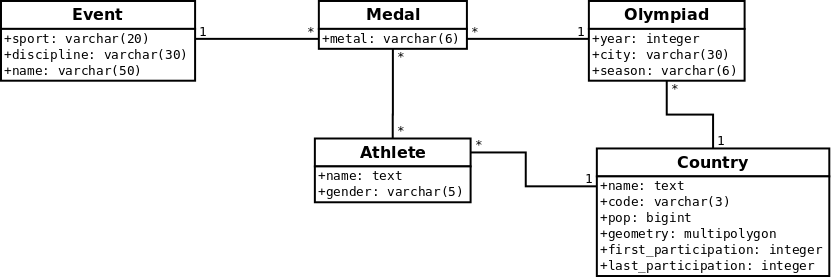
\includegraphics[width=\textwidth]{bdd.png}

\newpage

\subsubsection{Descriptif rapide de la base de données}

\begin{itemize}

\item
Une table \textit{event} contenant les épreuves pour lesquelles des médailles ont été décernées. Chacun des enregistrements (i.e. chaque épreuve) a :

\begin{itemize}

\item un sport \textit{sport}

\item une discipline \textit{discipline}

\item un nom d'épreuve \textit{name}

\end{itemize}

{\footnotesize Découpage effectué par le CIO}

\item
Une table \underline{géométrique} \textit{country} répertoriant les pays/délégations participants aux Jeux Olympiques avec  

\begin{itemize}

\item un nom \textit{name}

\item le code CIO associé \textit{code}

\item sa population \textit{pop}

\item sa première particiaption aux JO \textit{first\_participation}

\item sa dernière particiaption aux JO \textit{last\_participation}

\item sa géométrie \textit{geometry} {\footnotesize (type : MultiPolygon, projection : 4326, dimension : 2) }

\end{itemize}

{\footnotesize NB : Certaines délégations ont été représentées géographiquement de façon fictive : IOP, ZZX}

\item
Une table \textit{olympiad} listant toutes les olympiades pendant lesquelles des médailles ont été décernées

\begin{itemize}

\item l'année de l'olympiade \textit{year}

\item la ville dans laquelle s'est déroulée l'olympiade \textit{city}

\item la saison de l'olympiade \textit{season}

\item \textbf{l'identifiant du pays} \textit{country\_id}

\end{itemize}

\item
Une table \textit{athlete} recensant tous les athlètes médaillés dans une olympiade avec 

\begin{itemize}

\item le nom de l'athlète \textit{name}

\item son sexe \textit{gender}

\item \textbf{l'identifiant du pays pour lequel il a participé} \textit{country\_id}

\end{itemize}

\item
Une table \textit{medal} avec toutes les médailles décernées lors des Jeux Olympiques.

\begin{itemize}

\item le métal de la médaille \textit{metal}

\item \textbf{l'identifiant de l'athlète auquel la médaille a été remise} \textit{athlete\_id}

\item \textbf{l'identifiant de l'olympiade pendant laquelle la médaille a été remise} \textit{olympiad\_id}

\item \textbf{l'identifiant de l'épreuve pour laquelle la médaille a été remise} \textit{event\_id}

\end{itemize}

\end{itemize}

\subsection{Cadre technique}

Sont imposées dans la réalisation de votre projet :

\begin{itemize}

\item l'utilisation d'une bibliothèque cartographique : \textit{OpenLayers} ou \textit{Leaflet}

\item la récupération d'un ou plusieurs flux \textit{WMS}/\textit{TMS} externes (\textit{OSM}, \textit{Stamen} ...)

\item la création d'un ou plusieurs flux \textit{WFS} se reposant sur la base de données grâce à un \textit{GeoServer}

\item l'exposition cartographique de ces flux 

\end{itemize}

\newpage

\subsection{Fonctionnalités}

Sont attendues :
\begin{itemize}

\item la visualisation de la répartition des médailles (avec filtres : épreuve, nationalité, sexe ...)

\item la consultation des résultats par athlète, par délégation...

\item ...

\end{itemize}

Toute autre fonctionnalité vous paraissant intéressante pour votre site peut être développée : l'influence du pays hôte sur les résultats, le respect de la parité homme/femme, l'Histoire via les pays participants aux JO, \textit{insert here any good idea}...

Si votre site raconte une histoire, c'est mieux ! Il faut trouver une direction, un thème à votre application. 

Appropriez-vous le sujet pour éviter de développer une suite de fonctionnalités.

\subsection{Ouvertures possibles}

Les ouvertures ci-dessus ne sont pas prioritaires (ni personnelles), mais la richesse d'une application se situe dans les petits détails.

\begin{itemize}

\item l'administration de la base de données (ex: fonctionnalités de mise à jour)

\item la comparaison de cartes pour différentes années (ex: sur une même page, au passage de la souris ou autre)

\item la récupération et l'intégration d'autres données (ex: tracés des trajets des flammes olympiques)

\item ...

\end{itemize}

\section{Lancement du projet}

Au début du projet, vous avez récupéré un script \textbf{\textit{start.php}} ainsi qu'un dump sql permettant de créer et remplir la base de données.

Une fois la base de données chargée, il est fortement conseillé de s'amuser un peu avec, afin de bien la prendre en main.

\section{Liens utiles}

\begin{itemize}

\item
\href{https://www.lemonde.fr/les-decodeurs/article/2018/02/26/jo-2018-et-si-on-revoyait-le-classement_5262807_4355770.html}{Vu par le Monde}

\item
\href{http://www.wedodata.fr/equipe-jo2016.php}{Vu par l'Équipe}

\item
\href{https://www.bbc.com/sport/olympics/37148372}{Vu par la BBC}

\item
\href{https://www.statista.com/topics/1730/olympic-summer-games/}{Vision statistique}

\item
\href{https://www.theguardian.com/commentisfree/2012/aug/03/london-2012-olympics-open-data}{Version 2012}

\end{itemize}

\section{Conseils}

\begin{itemize}

\item Ne pas se lancer tête la première sans avoir trouvé un fil conducteur (et le conserver une fois acquis)

\item Structurer proprement son projet

\item Garder un code clair, organisé, bien indenté (pour faciliter la relecture)

\item Ne pas abuser du copier/coller

\item Demander de l'aide en cas de blocage

\end{itemize}

\end{document}
